%%%%%%%%%%%%%%%%%%%%%%%%%%%%%%%%%%%%%%%%
%%%%%  xPhO LaTeX Beamer Template  %%%%%
%%%%%  Date: 17/03/2025            %%%%%
%%%%%  Authors:                    %%%%%
%%%%%       Nguyen Thanh Long      %%%%%
%%%%%       Nguyen Le Mai Huong    %%%%%
%%%%%       Nguyen Minh Phuong     %%%%%
%%%%%%%%%%%%%%%%%%%%%%%%%%%%%%%%%%%%%%%%

\documentclass[aspectratio=169, t]{beamer} % Ratio 16:9
\usepackage[T5]{fontenc}
\usepackage{lmodern}
\usepackage{graphicx} 
\usepackage{array}
\usepackage{longtable} % for long table

\usepackage{amsmath}

\usepackage{chngcntr}
\counterwithin{figure}{section}

\renewcommand{\familydefault}{\sfdefault} % Font

\usepackage{caption}
\usepackage{siunitx}
\usepackage{mdframed}


% \definecolor{BlueDefault}{rgb}{0.2,0.2,0.7}
\definecolor{BlueDefault}{RGB}{14,47,95}


% Hide navigation 
\setbeamertemplate{navigation symbols}{}

% Setup background
\newcommand{\normalbackground}{%
    \usebackgroundtemplate{
\includegraphics[width=\paperwidth,height=\paperheight]{Background/Normal_slide_xPhO.pdf}}%
}

\newcommand{\titlebackground}{%
    \usebackgroundtemplate{
\includegraphics[width=\paperwidth,height=\paperheight]{Background/Title_slide_xPhO.pdf}}%
}

% Change the title color to white
\setbeamercolor{frametitle}{fg=white} 

% push the title up by \raisebox
\setbeamertemplate{frametitle}{%
    \vspace{0.3em}
    \hspace{-1em} \insertframetitle
    % \vspace{2mm}
}

% Number of slide
\setbeamertemplate{footline}{%
    \hfill
    \insertframenumber/\inserttotalframenumber
    \hspace{7.5mm}
    \vspace{3.5mm}
}

%% Make Table of Contents %%
\AtBeginSection[]{
  \begin{frame}
  \frametitle{Mục lục}
  \tableofcontents[currentsection]
  \end{frame}
}

%% Section numbering %%
\setbeamertemplate{section in toc}[sections numbered]
\setbeamertemplate{subsection in toc}[subsections numbered]


\renewcommand{\figurename}{Hình}
\renewcommand{\tablename}{Bảng}


%%%%% Bibliography %%%%%
\usepackage[backend=biber,style=ieee]{biblatex}
\addbibresource{citation.bib}

\usepackage{url}
\usepackage{hyperref}
\hypersetup{
	colorlinks=true,
	linkcolor=BlueDefault,
	filecolor=BlueDefault,
    citecolor=BlueDefault,
	urlcolor=BlueDefault,
	pdftitle={Overleaf Example},
	pdfpagemode=FullScreen,
}

%tikz
\usepackage{tikz}


\begin{document}

\titlebackground

\begin{frame}[noframenumbering]
    \thispagestyle{empty}
    \bfseries
    \begin{flushleft}
        \vfill
        \vspace{5mm}
        \textcolor{BlueDefault}{\huge \bfseries Vector và  \\Nhập môn Đại số tuyến tính} \\
        \vspace{8mm}
        \textcolor{black}{\large \bfseries Người trình bày: Carina }
        \vfill
    \end{flushleft}
\end{frame}

\normalbackground

\section{Nguyên hàm và tích phân}

\begin{frame}{Ý nghĩa của phương trình vi phân trong bài toán chuyển động}
    %Dẫn từ phương trình vi phân => cần phép toán nguyên hàm và tích phân.

    %y'=f(x) =? y(x) = ?

    %Nguyên hàm, xác định hằng số C

    %Chúng ta đã biết về phép đạo hàm, nhưng có phép nào làm ngược lại quá trình không?
    \begin{center}
    \begin{minipage}{0.45\linewidth}
    \begin{figure}
        \centering
        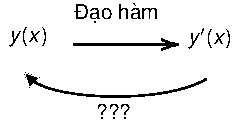
\includegraphics[width=0.6\linewidth]{Figures/Int_1.pdf}
        \label{fig:Int_1}
    \end{figure}
    \end{minipage}
    \hspace{1mm}
    \begin{minipage}{0.4\linewidth}
        Giải phương trình vi phân
        \begin{equation*}
            y'(x) = f(x).
        \end{equation*}
    Sử dụng 
    \vspace{-2mm}
    
    \begin{equation*}
        dy = f(x) dx.
    \end{equation*}
    \end{minipage}
    \end{center}
    Ta định nghĩa một phép toán ngược quá trình đạo hàm. Ký hiệu là \("\displaystyle \int "\). Sao cho
    \vspace{1mm}
    
    \begin{equation}
        \int f(x) dx = y(x) + C \ \ \ \ \text{,Với \(C\) là hằng số}.
        \label{eq:int_1}
    \end{equation}
    
    Ta gọi phép toán ở (\ref{eq:int_1}) là nguyên hàm.
\end{frame}

\begin{frame}{Bài toán diện tích và phương pháp vét cạn}
\begin{center}
    \begin{minipage}{0.45 \linewidth}
        \begin{figure}
            \centering
            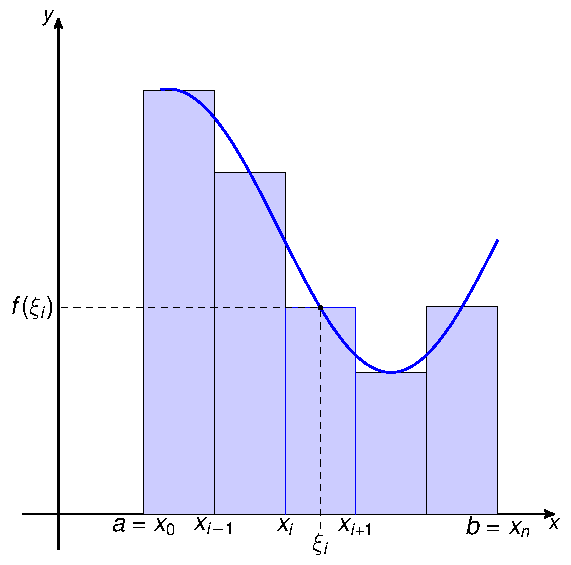
\includegraphics[width=1\linewidth]{Figures/Int_2.pdf}
            \label{fig:Int_2}
        \end{figure}
    \end{minipage}
    \begin{minipage}{0.45\linewidth}
        \begin{figure}
            \centering
            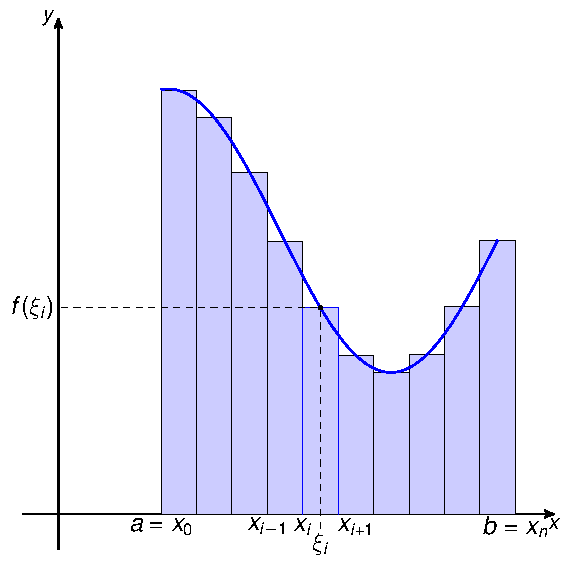
\includegraphics[width=1\linewidth]{Figures/Int_3.pdf}
            \label{fig:Int_3}
        \end{figure}   
    \end{minipage}
\end{center}

\end{frame}
\begin{frame}{Bài toán diện tích và phương pháp vét cạn}
    \begin{center}
        \begin{minipage}{0.4\linewidth}
        \begin{figure}
            \centering
            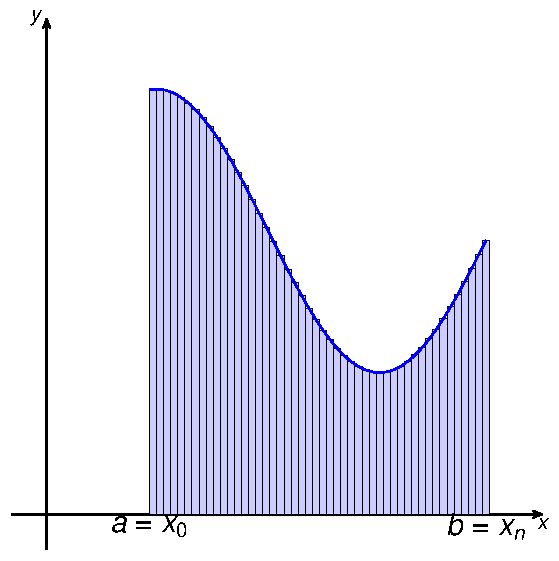
\includegraphics[width=1\linewidth]{Figures/Int_4.pdf}
            \caption{Khi ta chia đủ nhỏ}
            \label{fig:Int_4}
        \end{figure}
        \end{minipage}
        \hspace{1mm}
        \begin{minipage}{0.4\linewidth}
            Diện tích 
            \begin{equation}
            \label{eq:int_2}
            \begin{split}
                &S \simeq  \sum_{i=0}^n f(\xi_i) \Delta x \\
                &\text{Với}
                \left\{
                \begin{array}{ccc}
                \Delta x &=& x_{i+1} - x_i \\
                \xi_i &\in& [x_i,x_{i+1}]
                \end{array}
                \right.
            \end{split}
            \end{equation}  
            Đây là công thức tổng Riemann để xấp xỉ diện tích bên dưới đồ thị.
        \end{minipage}
    \end{center}
\end{frame}
\begin{frame}{Mối liên hệ nguyên hàm - tích phân}
    Ở công thức (\ref{eq:int_2}), ta có thể chọn tuỳ ý \(\xi_i\). Nên ta chọn \(\xi_i = x_i\). Lúc này
    \begin{equation*}
        S \simeq \sum_{i=0}^n f(x_i) \Delta x.   
    \end{equation*}
    Nếu ta lấy giới hạn sao cho các cột diện tích đủ nhỏ thì ta sẽ có
    \begin{equation}
        \displaystyle
        \Delta x \rightarrow dx \ \text{thì} \ \sum_{i=0}^n \rightarrow \int_{a}^b
        \label{eq:int_3}
    \end{equation}
\end{frame}
\begin{frame}{Ví dụ}
    Cho một vật di chuyển với đồ thị vận tốc \(v = f(t) = at+b\). Tìm quãng đường nó di chuyển được trong thời gian \(t \in [c,d]\). Tìm diện tích trong khoảng \(t \in [c,d]\).
    \begin{center}
                    \underline{Giải}
    \end{center}
    \begin{center}
        \begin{minipage}{0.35\linewidth}
            \begin{figure}
                \centering
                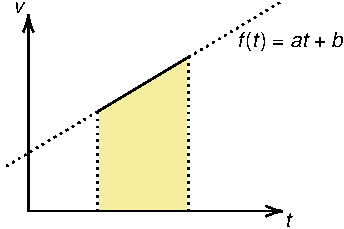
\includegraphics[width=1\linewidth]{Figures/Int_5.pdf}
                \label{fig:Int_5}
            \end{figure}
        \end{minipage}
        \hspace{1mm}
        \begin{minipage}{0.5\linewidth}

            Quãng đường: 
            \begin{equation*}
                \Delta x = \int_{c}^{d} f(t) dt = \frac{a}{2} (d^2-c^2) + b(d-c).
            \end{equation*}
            Diện tích: Đây là diện tích hình thang vuông.
            \begin{equation*}
            \begin{split}
                \Delta S &= \frac12 \left(f(d) + f(c)\right) (d-c) \\&=  \frac{a}{2} (d^2-c^2) + b(d-c).             
            \end{split}
            \end{equation*}
        \end{minipage}
    \end{center}
\end{frame}
\begin{frame}{Nguyên hàm và tích phân, định lý Leibniz–Newton}


    Định lý Leibniz–Newton

    \begin{mdframed}[backgroundcolor=BlueDefault!10, linecolor=BlueDefault, linewidth=1pt]
    Nếu nguyên hàm của \(f(x)\) là \(F(x)\) thì 
    \begin{equation}
        \int_{a}^{b} f(x) dx = F(b) - F(a).      
    \end{equation}
    \end{mdframed}
    

    
\end{frame}

\begin{frame}{Giải phương trình vi phân: phân ly biến số}
    Phương pháp phân ly biến số dùng để giải quyết các phương trình vi phân cơ bản.
    \begin{equation*}
        f(x,y,y') = 0 .
    \end{equation*}
    Tách biến có nghĩa là mỗi vế của phương trình sẽ chỉ chứa một biến
    \begin{equation}
        f(x,y,y') = 0  \longrightarrow h(y) y' = g(x) \Longrightarrow{h(y) dy = g(x) dx}
    \end{equation}
    Ví dụ: Cho phương trình vi phân


    \begin{center}
        \begin{minipage}{0.45\linewidth}
            \begin{equation*}
                \begin{array}{ccl}
                &\displaystyle \frac{dv}{dt} &= -bv \\
                \pause 
                \\
                \Longrightarrow &\displaystyle \frac{dv}{v} &= -b dt \\
                \end{array} 
            \end{equation*}
        \end{minipage}
        \hspace{1mm}
        \begin{minipage}{0.5\linewidth}
            \begin{equation*}
                \begin{array}{ccl}
                \Longrightarrow &\displaystyle \int_{v_0}^{v(t)} \frac{dv}{v} &=\displaystyle  -\int_{0}^{t} b dt \\
                \\
                \Longrightarrow & \ln (v(t)/v_0)  &= -bt \\
                \end{array}  
            \end{equation*}
        \end{minipage}
    \end{center}
\end{frame}

\section{Hệ tọa độ}

\subsection{Hệ tọa độ và các hệ tọa độ phổ biến}

\begin{frame}{Ý nghĩa của hệ tọa độ}
    \begin{columns}
        \column{0.32\textwidth}
        \begin{itemize}
            \item Xác định vị trí các vật trong không gian.
            \item Các trục, biến tọa độ được tùy chọn phù hợp với từng ví dụ.
            \item Các hệ tọa độ trực giao thường được ưu tiên sử dụng với các hệ phức tạp.
        \end{itemize}
        \column{0.68\textwidth}
        \vspace{-4mm}
        \begin{figure}
            \centering
            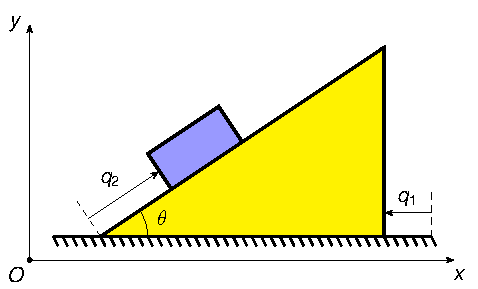
\includegraphics[width=0.9\linewidth]{Figures/Sliding_wedge.pdf}
            \caption{Nhiều hệ tọa độ khác nhau cho bài toán nêm trượt trên nêm}
            \label{fig:Sliding_wedge}
        \end{figure}
    \end{columns}
\end{frame}

\begin{frame}{Các hệ tọa độ 3 chiều phổ biến}
    \vspace{-4mm}
    \begin{columns}
        \column{0.33\textwidth}
        \begin{itemize}
            \item Hệ tọa độ Dercates
        \end{itemize}
        \begin{figure}
            \centering
            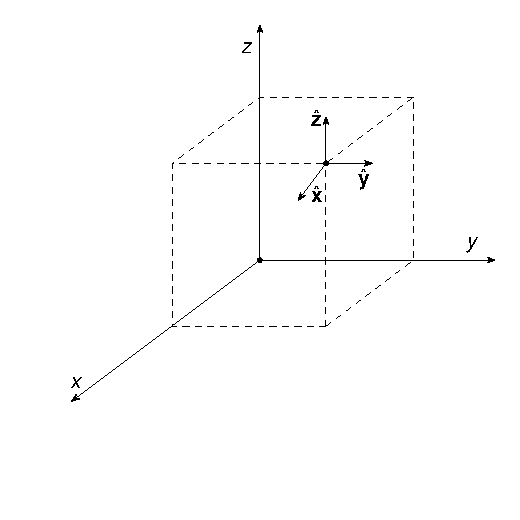
\includegraphics[width=\linewidth]{Figures/Decartes_coordinate.pdf}
            \caption{Hệ tọa độ Decartes.}
            \label{fig:Decartes_coordinate}
        \end{figure}

        \column{0.33\textwidth}
        \begin{itemize}
            \item Hệ tọa độ trụ
        \end{itemize}
        \begin{figure}
            \centering
            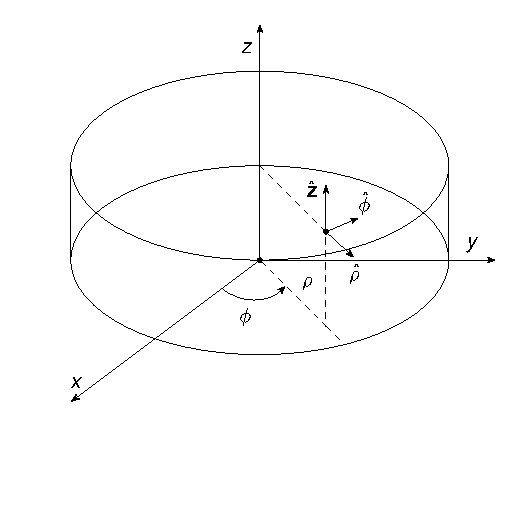
\includegraphics[width=\linewidth]{Figures/Cylindrical_coordinates.pdf}
            \caption{Hệ tọa độ trụ.}
            \label{fig:Cylindrical_coordinates}
        \end{figure}

        \column{0.33\textwidth}
        \begin{itemize}
            \item Hệ tọa độ cầu
        \end{itemize}
        \begin{figure}
            \centering
            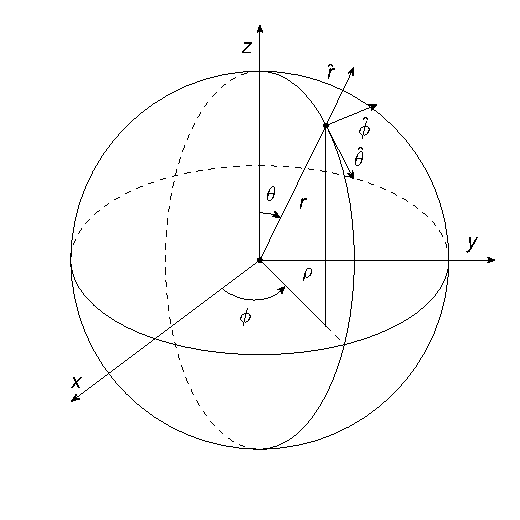
\includegraphics[width=\linewidth]{Figures/Spherical_coordinate.pdf}
            \caption{Hệ tọa độ cầu.}
            \label{fig:Spherical_coordinate}
        \end{figure}

    \end{columns}

\end{frame}

\begin{frame}{Tọa độ Frenet - Serret}
    \begin{columns}
        \column{0.33\textwidth}
            Tên gọi
            \begin{itemize}
                \item Vector đơn vị tiếp tuyến \(\mathbf{T}\).
                \item Vector đơn vị pháp tuyến \(\mathbf{N}\).
                \item Vector đơn vị trực chuẩn \(\mathbf{B}\).
            \end{itemize}
        \column{0.33\textwidth}
            Định nghĩa:
            \begin{align}
                \mathbf{T} & := \frac{\mathrm{d} \mathbf{r}}{\mathrm{d} s}, \\
                \mathbf{N} & := \frac{\mathrm{d} \mathbf{T} / \mathrm{d} s}{\left\| \mathrm{d} \mathbf{T} / \mathrm{d} s \right\|}, \\
                \mathbf{B} & := \mathbf{T} \times \mathbf{N}.
            \end{align}
        \column{0.33\textwidth}
            Công thức Frenet Serret
            \begin{align}
                \frac{\mathrm{d} \mathbf{T}}{\mathrm{d} s} &= \kappa \mathbf{N}, \\
                \frac{\mathrm{d} \mathbf{N}}{\mathrm{d} s} &= - \kappa \mathbf{T} + \tau \mathbf{B}, \\
                \frac{\mathrm{d} \mathbf{B}}{\mathrm{d} s} &= - \tau \mathbf{N}.
            \end{align}
    \end{columns}
    \begin{columns}
        \column{0.33\textwidth}
        \begin{itemize}
            \item Độ cong \(\kappa\).
            \item Bán kính cong \(R_c = 1/\kappa\).
            \item Độ xoắn đường cong không gian \(\tau\).
        \end{itemize}
        \column{0.67\textwidth}
        \vspace{-2mm}
        \begin{figure}
            \centering
            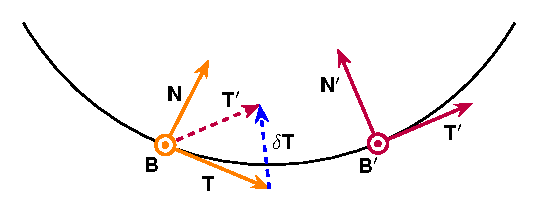
\includegraphics[width=0.7\linewidth]{Figures/Frenet_Serret.pdf}
            \vspace{-2mm}
            \caption{Các vector đơn vị trên hệ tọa độ cong.}
            \label{fig:Frenet_Serret}
        \end{figure}
    \end{columns}
\end{frame}

\subsection{Độ cong và bán kính cong}

\begin{frame}{Tính toán bán kính cong trong không gian 2 chiều - đường cycloid}
    \begin{columns}
        \column{0.6\textwidth}
            Độ cong:
            \begin{equation}
                \kappa = \dfrac{\mathrm{d} \phi}{\mathrm{d} s} = \frac{x' y" - y' x"}{\left( x'^2 + y'^2 \right)^{3/2}}
            \end{equation}
            Bán kính cong \(R_c = 1/\kappa\), tính toán với đường cycloid
            \begin{equation}
                R_c = 4 R \cos \left( \dfrac{\theta}{2} \right).
            \end{equation}
            Tại điểm cao nhất, \(\theta=0\), \(R_c=4R\).
            \begin{itemize}
                \item Bán kính cong là bán kính của đường tròn khớp nhất so với quỹ đạo tại điểm được khảo sát. \cite{BoiDuoongHSGTHPT_Phantich}
            \end{itemize}
        \column{0.4\textwidth}
        \vspace{-7mm}
        \begin{figure}
            \centering
            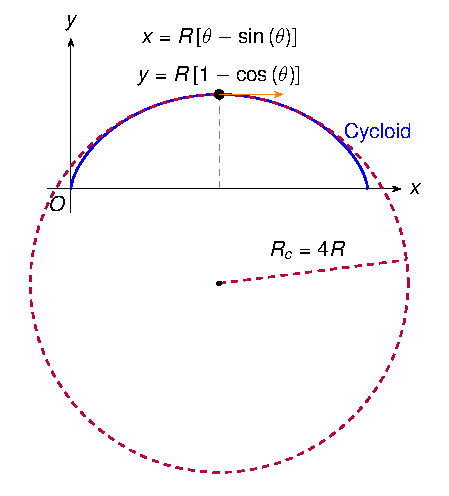
\includegraphics[width=0.9\linewidth]{Figures/Cycloid.pdf}
            \caption{Quỹ đạo Cycloid và bán kính cong tại điểm cao nhất trên quỹ đạo.}
            \label{fig:Cycloid}
        \end{figure}
    \end{columns}
\end{frame}

\subsection{Chuyển động ném xiên}

\begin{frame}{Chuyển động ném xiên}
    \begin{columns}
        \column{0.5\textwidth}
        \vspace{-3mm}
            \begin{itemize}
                \item Điều kiện đầu: \\
                \(x(0)=0\), \(y(0)=0\), \(\dot{x}(0)= v_0 \cos \alpha\), \(\dot{y}(0)= v_0 \sin \alpha\).
                \item Phương trình vi phân chuyển động: \(\ddot{x} = 0\), \(\ddot{y} = -g\).
                \item Nghiệm:
                \begin{align}
                    x(t) &= v_0 \cos \left( \alpha \right) t, \\
                    y(t) &= v_0 \sin \left( \alpha \right) t - \frac{1}{2} g t^2 \\
                    y(x) &= x \tan \left( \alpha \right) - \frac{v_0^2}{2g \cos^2 \left( \alpha \right)}x^2. 
                \end{align}
            \end{itemize}            
        \column{0.5\textwidth}
            \vspace{-2mm}
            \begin{figure}
                \centering
                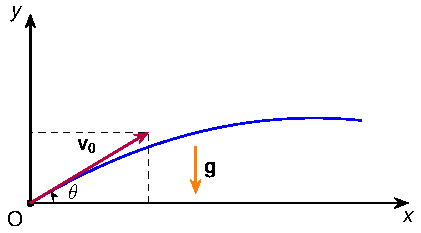
\includegraphics[width=0.9\linewidth]{Figures/Projectile_motion.pdf}
                \caption{Bài toán chuyển động ném xiên, các điều kiện đầu và quỹ đạo của vật.}
                \label{fig:Projectile_motion}
            \end{figure}
            \vspace{-5mm}
            \begin{itemize}
                \item Bài tập: Xác định độ cong và bán kính cong của quỹ đạo tại thời điểm \(t\).
            \end{itemize}
    \end{columns}
\end{frame}

\subsection{Bài toán đuổi bắt}

\begin{frame}{Bài toán đuổi bắt - 1: Rùa đuổi nhau}
    \begin{columns}
        \column{0.3\textwidth}
            Giải
            \begin{align*}
                r \frac{\mathrm{d} \theta}{\mathrm{d} r} &= -1 \\
                \int_{a/\sqrt{2}}^r \frac{\mathrm{d} r}{r} &= - \int_{\pi/4}^\theta \mathrm{d} \theta  \\
                \Rightarrow r &= \frac{a}{\sqrt{2}} \exp \left( \frac{\pi}{4} -\theta \right).
            \end{align*}

            \begin{itemize}
                \item Tỷ lệ vàng!!!
            \end{itemize}
        \column{0.7\textwidth}
        \begin{figure}
            \centering
            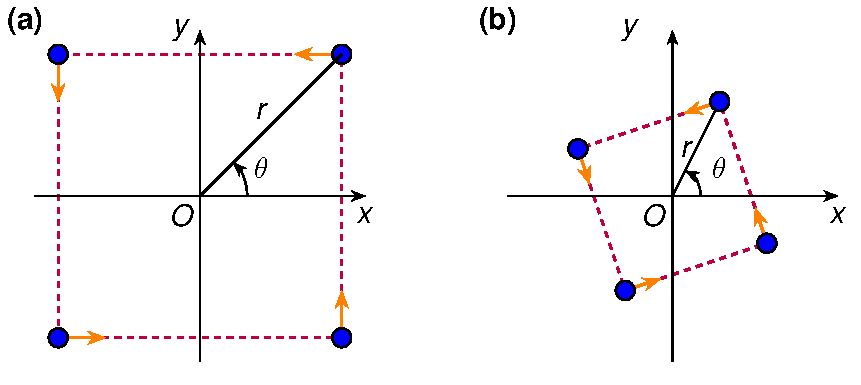
\includegraphics[width=0.9\linewidth]{Figures/Turtles_ninja.pdf}
            \caption{4 con rùa đuổi bắt: \textbf{(a)} Thời điểm ban đầu, \textbf{(b)} Tại một thời điểm bất kỳ}
            \label{fig:Turtles_ninja}
        \end{figure}
    \end{columns}
\end{frame}

\begin{frame}{Bài toán đuổi bắt - 2: Chó đuổi thỏ}
    \begin{columns}
        \column{0.3\textwidth}
            Viết phương trình vi phân đối với hai hệ tọa độ khác nhau:
            \begin{itemize}
                \item Tọa độ Decartes \( \left( x, y \right) \).
                \item Toạ độ cực \( \left( r, \theta \right) \). \cite{brebec2005cohoc1}
            \end{itemize}
        \vspace{5mm}
        \textit{Giải phương trình vi phân của bài toán này sẽ là một câu chuyện khác...}
        \column{0.7\textwidth}
        \vspace{-5mm}
        \begin{figure}
            \centering
            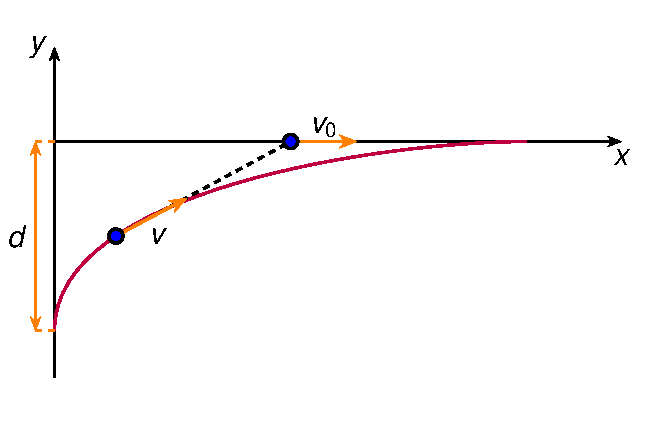
\includegraphics[width=0.9\linewidth]{Figures/Pursuit.pdf}
            \vspace{-2mm}
            \caption{Chó vận tốc \(v\) đuổi theo thỏ chuyển động thẳng vận tốc \(v_0\).}
            \label{fig:Pursuit}
        \end{figure}
    \end{columns}
\end{frame}



\section{Hệ quy chiếu}

\subsection{Hệ quy chiếu quán tính - phi quán tính}
\begin{frame}{Hệ quy chiếu}
    %Phân biệt giữa các hệ quy chiếu có cùng vận tốc tức thời, nhưng khác về gia tốc (và các đạo hàm bậc cao)
    \begin{center}
        \begin{minipage}[t]{0.45\linewidth}
            \begin{figure}[!htb]
                \centering
                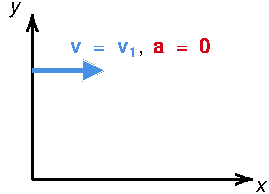
\includegraphics[width=0.9\linewidth]{Figures/FoR_1.pdf}
                \caption{Hệ quy chiếu quán tính}
                \label{fig:FoR_1}
            \end{figure}
        \end{minipage}
        \hspace{5mm}
        \begin{minipage}[t]{0.45\linewidth}            
            \begin{figure}[!htb]
                \centering
                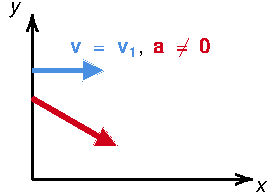
\includegraphics[width=0.9\linewidth]{Figures/FoR_2.pdf}
                \caption{Hệ quy chiếu phi quán tính}
                \label{fig:FoR_2}
            \end{figure}
        \end{minipage}
    \end{center}
\end{frame}

\subsection{Định lý cộng vận tốc và gia tốc}

\begin{frame}{Định lý cộng vận tốc và cộng gia}
    %Chỉ dựa trên công thức

    %Ví dụ: chỉ liên hệ giữa tịnh tiến

    Xét một điểm M trong hệ quy chiếu \(O_1\). Ta sẽ biểu diễn toạ độ, vận tốc, gia tốc của M trong hệ quy chiếu \(O\).

    \begin{center}
        \begin{minipage}{0.4\linewidth}
            \begin{figure}[!htb]
                \centering
                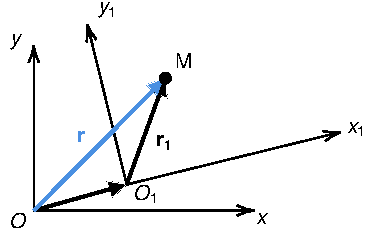
\includegraphics[width=1\linewidth]{Figures/FoR_3.pdf}
                \caption{}
                \label{fig:FoR_3}
            \end{figure}        
        \end{minipage}
        \hspace{1mm}
        \begin{minipage}{0.45\linewidth}
        \begin{equation*}
                \begin{array}{cl}
                \text{Toạ độ} &\left\{
                \begin{array}{cl}
                (O_1): &\mathbf{r_1} \\
                (O): &\mathbf{r} = \mathbf{OO_1} + \mathbf{r_1}
                \end{array}
                \right. 
                \\
                \\
                \text{Vận tốc} &\left\{
                \begin{array}{cl}
                (O_1): &\dot{\mathbf{r}}_1 \\
                (O): &\dot{\mathbf{r}} = \displaystyle \frac{d}{dt}\mathbf{OO}_1 + \dot{\mathbf{r}}_1
                \end{array}
                \right.
                \\
                \\
                \text{Gia tốc} &\left\{
                \begin{array}{cl}
                (O_1): &\ddot{\mathbf{r}}_1 \\
                (O): &\ddot{\mathbf{r}} =\displaystyle \frac{d^2}{dt^2} \mathbf{OO}_1 + \ddot{\mathbf{r}}_1
                \end{array}
                \right.
                \end{array}
        \end{equation*}
        \end{minipage}
    \end{center}
\end{frame}
\begin{frame}{Ví dụ}
    Cho một bánh quay (tâm \(O_1\) cố định), ta đặt hệ quy chiếu ở các điểm \(O,O_1,A,B\). Bánh quay với vận tốc góc \(\omega\), bán kính \(R\).
\begin{center}
    \begin{minipage}{0.5\linewidth}
        \begin{figure}
        \centering
        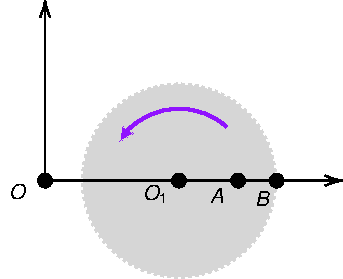
\includegraphics[width=0.8\linewidth]{Figures/FoR_4.pdf}
        \caption{}
        \label{fig:FoR_4}
        \end{figure}        
    \end{minipage}
    \hspace{1mm}
    \begin{minipage}{0.4\linewidth}
        \begin{equation*}
            \begin{array}{ll}
            \mathbf{v_{O_1/B}} &= \mathbf{\omega} \times \mathbf{BO_1} \\ \\
            \mathbf{v_{B/A}} &= \mathbf{\omega} \times \mathbf{BA} \\ \\
            \mathbf{v_{B/O}} &= \mathbf{(-\omega)} \times \mathbf{BO} 
            \end{array}
        \end{equation*}         
    \end{minipage}
\end{center}
\end{frame}







\begin{frame}[allowframebreaks]{Tài liệu tham khảo}
    \begin{refsection}
        \nocite{morin2008introduction,calculusjame, 3b1b,griffiths2023introduction}
         \printbibliography
    \end{refsection}
\end{frame}

\end{document}